% 图 15.1 —— 由 `checks/emit_hand.py` 自动拼出（probe 精测 + prims2 图元分解）
%%
% ⚠ 这是**稿子不是成品**：跑 `checks/checkhand.py 15.1` 看指标 + 看叠合图。
%%
%% ⚠ 待核：
%   · 本图 probe 报出阴影族 1 个 —— **本脚本不生成阴影**（要照原书手写）；prims2 的 strokes 里可能含阴影线，核对时留意别画重
%   · 可疑字形 1 项（空心圈 ⊙ 常被认成字母 o）—— 见文件末
%%
\documentclass[12pt]{standalone}
\usepackage{fontspec}
\setsansfont{Arial}
\newfontfamily\mfallback{DejaVu Sans}
\usepackage{tikz}
\begin{document}
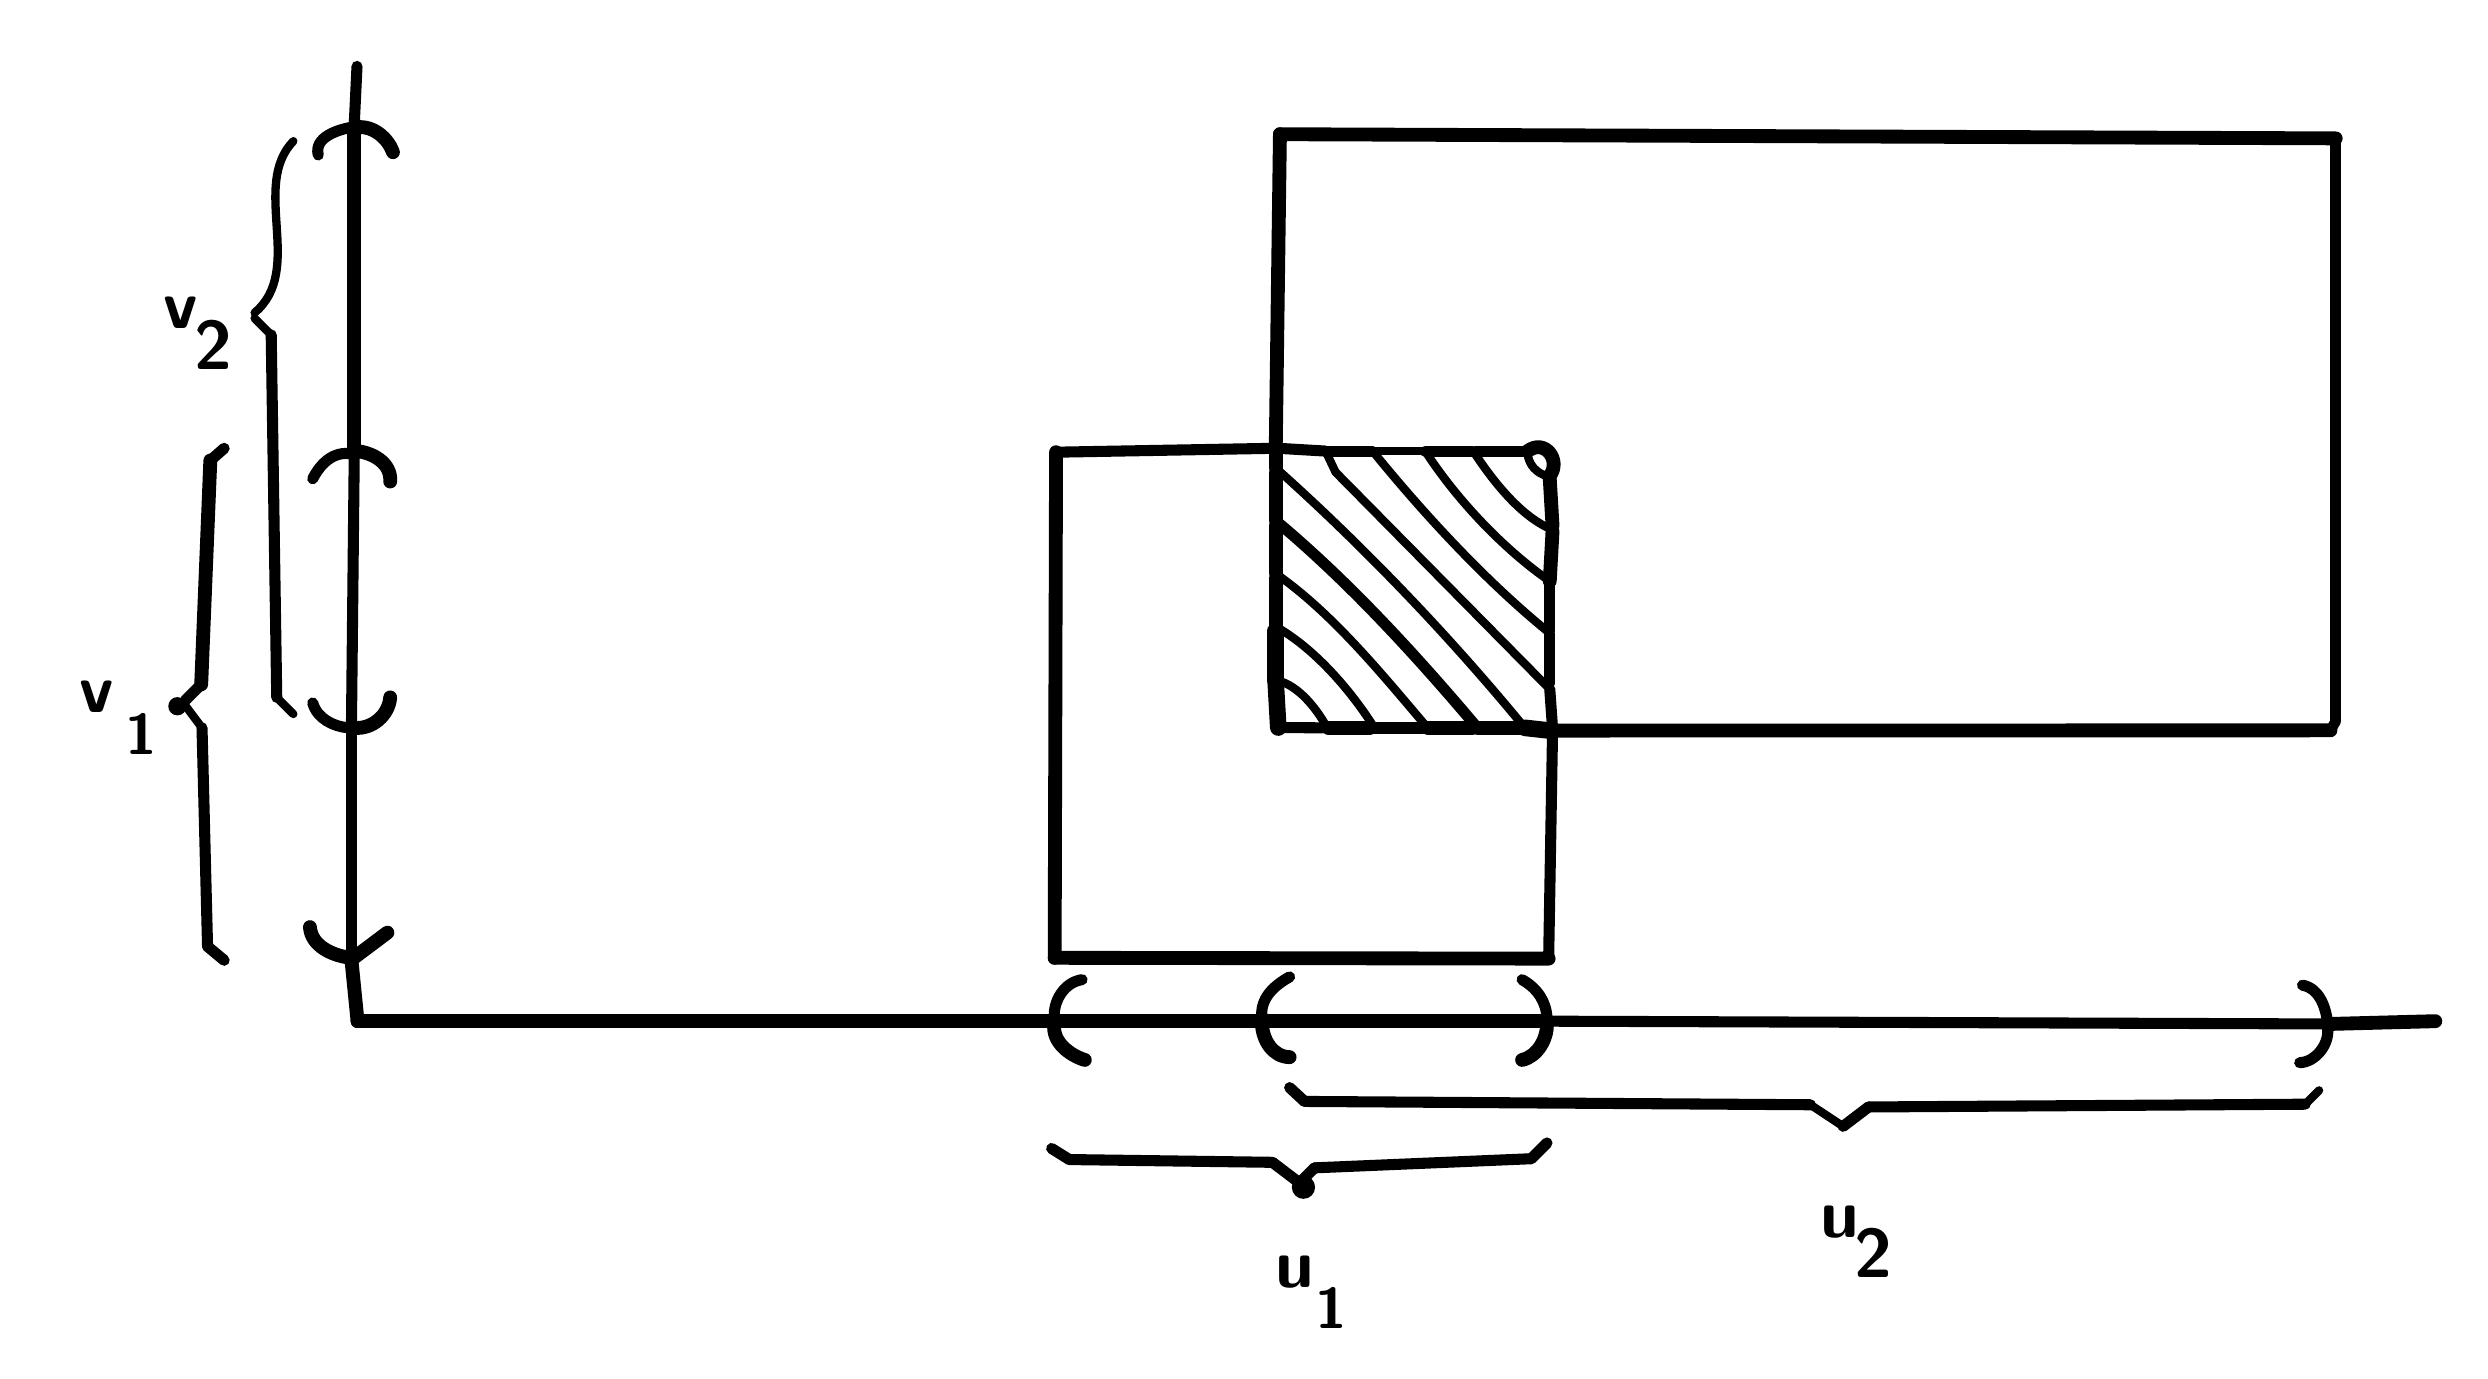
\begin{tikzpicture}[x=1pt, y=-1pt, line width=4.0pt, line cap=round, line join=round]

  %% ════ 填充区（prims2 的 fills）════

  %% ════ 直线段（prims2 的 strokes）════
  \draw[line width=4.0pt] (830.0,360.0) -- (550.0,359.0);
  \draw[line width=6.0pt] (550.0,254.0) -- (541.0,253.0);
  \draw[line width=4.5pt] (487.0,253.0) -- (504.0,253.0);
  \draw[line width=4.0pt] (551.0,253.0) -- (550.0,239.0);
  \draw[line width=5.0pt] (832.0,360.0) -- (870.0,359.0);
  \draw[line width=5.0pt] (552.0,254.0) -- (832.1,253.9);
  \draw[line width=3.8pt] (832.1,253.9) -- (834.0,250.6);
  \draw[line width=4.0pt] (834.0,250.6) -- (834.0,40.0);
  \draw[line width=5.0pt] (834.0,40.0) -- (452.5,38.5);
  \draw[line width=5.0pt] (452.5,38.5) -- (451.0,151.0);
  \draw[line width=4.0pt] (551.0,255.0) -- (549.6,336.4);
  \draw[line width=5.0pt] (549.6,336.4) -- (371.1,336.1);
  \draw[line width=5.0pt] (371.1,336.1) -- (371.6,153.4);
  \draw[line width=4.0pt] (371.6,153.4) -- (450.0,152.0);
  \draw[line width=5.0pt] (550.0,163.0) -- (551.0,180.0);
  \draw[line width=5.0pt] (370.0,359.0) -- (119.2,359.0);
  \draw[line width=5.0pt] (119.2,359.0) -- (117.0,337.0);
  \draw[line width=4.0pt] (57.0,243.0) -- (62.7,237.3);
  \draw[line width=5.0pt] (62.7,237.3) -- (66.0,156.4);
  \draw[line width=4.0pt] (66.0,156.4) -- (71.0,152.0);
  \draw[line width=6.0pt] (451.0,218.0) -- (451.0,236.0);
  \draw[line width=5.0pt] (372.0,359.0) -- (445.0,359.0);
  \draw[line width=4.0pt] (523.0,153.0) -- (541.0,153.0);
  \draw[line width=4.0pt] (486.0,153.0) -- (469.0,153.0);
  \draw[line width=3.0pt] (486.0,153.0) -- (505.0,153.0);
  \draw[line width=4.0pt] (117.0,335.0) -- (117.0,254.0);
  \draw[line width=5.0pt] (548.0,359.0) -- (447.0,359.0);
  \draw[line width=6.0pt] (451.0,237.0) -- (451.9,252.9);
  \draw[line width=4.0pt] (451.9,252.9) -- (468.0,253.0);
  \draw[line width=5.0pt] (451.0,197.0) -- (451.0,180.0);
  \draw[line width=5.0pt] (118.0,336.0) -- (130.0,327.0);
  \draw[line width=5.0pt] (541.0,253.0) -- (524.0,253.0);
  \draw[line width=5.0pt] (451.0,199.0) -- (451.0,216.0);
  \draw[line width=4.0pt] (549.0,403.0) -- (543.3,408.7);
  \draw[line width=4.0pt] (543.3,408.7) -- (465.0,412.0);
  \draw[line width=4.0pt] (465.0,412.0) -- (460.0,417.0);
  \draw[line width=3.0pt] (57.0,245.0) -- (63.0,253.0);
  \draw[line width=4.0pt] (63.0,253.0) -- (65.0,332.0);
  \draw[line width=4.0pt] (65.0,332.0) -- (71.0,337.0);
  \draw[line width=5.0pt] (451.0,161.0) -- (451.0,178.0);
  \draw[line width=5.0pt] (470.0,253.0) -- (485.0,253.0);
  \draw[line width=4.0pt] (117.0,252.0) -- (118.0,155.0);
  \draw[line width=4.0pt] (459.0,417.0) -- (449.8,410.0);
  \draw[line width=4.0pt] (449.8,410.0) -- (376.4,409.0);
  \draw[line width=4.0pt] (376.4,409.0) -- (370.0,405.0);
  \draw[line width=4.0pt] (550.0,219.0) -- (550.0,237.0);
  \draw[line width=3.0pt] (828.0,384.0) -- (823.0,389.0);
  \draw[line width=4.0pt] (823.0,389.0) -- (665.2,390.0);
  \draw[line width=4.0pt] (665.2,390.0) -- (656.0,397.0);
  \draw[line width=4.0pt] (522.0,153.0) -- (505.0,153.0);
  \draw[line width=4.0pt] (456.0,383.0) -- (461.4,388.0);
  \draw[line width=4.0pt] (461.4,388.0) -- (644.2,389.2);
  \draw[line width=3.0pt] (644.2,389.2) -- (656.0,397.0);
  \draw[line width=4.0pt] (119.0,14.0) -- (118.0,35.0);
  \draw[line width=5.0pt] (451.0,153.0) -- (451.0,159.0);
  \draw[line width=5.0pt] (551.0,182.0) -- (550.0,200.0);
  \draw[line width=4.0pt] (550.0,200.0) -- (550.0,218.0);
  \draw[line width=3.0pt] (96.0,248.0) -- (90.0,242.0);
  \draw[line width=4.0pt] (90.0,242.0) -- (88.0,111.0);
  \draw[line width=3.0pt] (88.0,111.0) -- (82.0,105.0);
  \draw[line width=5.0pt] (522.0,253.0) -- (506.0,253.0);
  \draw[line width=5.0pt] (118.0,37.0) -- (118.0,152.0);
  \draw[line width=4.0pt] (452.0,152.0) -- (469.0,153.0);
  \draw[line width=3.0pt] (469.0,153.0) -- (472.6,160.6);
  \draw[line width=3.0pt] (472.6,160.6) -- (549.0,238.0);

  %% ════ 曲线（prims2 的 curves —— 三段式，坐标同为 (y,x)）════
  \draw[line width=4.0pt] (117.0,36.0) .. controls (112.0,36.9) and (103.4,39.6) .. (105.0,46.0);
  \draw[line width=5.0pt] (549.0,360.0) .. controls (549.1,365.4) and (545.6,371.7) .. (540.0,373.0);
  \draw[line width=3.0pt] (452.0,236.0) .. controls (459.2,237.9) and (465.5,245.8) .. (469.0,252.0);
  \draw[line width=5.0pt] (119.0,36.0) .. controls (124.8,35.3) and (130.2,39.9) .. (132.0,45.0);
  \draw[line width=4.0pt] (371.0,358.0) .. controls (370.4,351.8) and (374.6,344.9) .. (381.0,344.0);
  \draw[line width=4.0pt] (456.0,343.0) .. controls (450.4,346.1) and (445.1,350.8) .. (446.0,358.0);
  \draw[line width=3.0pt] (549.0,218.0) .. controls (526.4,199.5) and (504.4,175.6) .. (486.0,153.0);
  \draw[line width=4.0pt] (116.0,253.0) .. controls (110.6,252.6) and (104.6,249.7) .. (103.0,244.0);
  \draw[line width=5.0pt] (382.0,373.0) .. controls (376.7,371.4) and (370.0,366.5) .. (371.0,360.0);
  \draw[line width=5.0pt] (116.0,336.0) .. controls (110.2,335.2) and (102.5,331.9) .. (102.0,325.0);
  \draw[line width=5.0pt] (118.0,253.0) .. controls (124.4,253.6) and (130.5,248.5) .. (131.0,242.0);
  \draw[line width=4.0pt] (549.0,358.0) .. controls (548.8,352.0) and (545.5,347.1) .. (540.0,344.0);
  \draw[line width=4.0pt] (822.0,346.0) .. controls (828.1,347.1) and (830.3,353.9) .. (831.0,359.0);
  \draw[line width=3.0pt] (549.0,162.0) .. controls (545.2,161.0) and (542.4,157.9) .. (542.0,154.0);
  \draw[line width=4.0pt] (831.0,361.0) .. controls (832.1,366.9) and (826.9,373.8) .. (821.0,374.0);
  \draw[line width=4.0pt] (117.0,154.0) .. controls (110.3,152.9) and (105.7,157.7) .. (103.0,163.0);
  \draw[line width=3.0pt] (541.0,253.0) .. controls (514.4,220.6) and (483.5,188.2) .. (452.0,160.0);
  \draw[line width=3.0pt] (96.0,41.0) .. controls (80.4,57.2) and (100.3,87.7) .. (82.0,103.0);
  \draw[line width=3.0pt] (452.0,198.0) .. controls (471.7,212.0) and (489.2,233.4) .. (505.0,252.0);
  \draw[line width=3.0pt] (452.0,217.0) .. controls (465.4,224.9) and (477.8,239.2) .. (486.0,252.0);
  \draw[line width=3.0pt] (550.0,181.0) .. controls (539.2,176.2) and (529.5,163.8) .. (523.0,154.0);
  \draw[line width=5.0pt] (456.0,372.0) .. controls (449.8,371.9) and (446.2,365.6) .. (446.0,360.0);
  \draw[line width=4.0pt] (452.0,179.0) .. controls (477.6,200.5) and (501.6,226.7) .. (523.0,252.0);
  \draw[line width=3.0pt] (550.0,200.0) .. controls (533.1,188.3) and (516.1,170.2) .. (505.0,153.0);
  \draw[line width=5.0pt] (550.0,162.0) .. controls (554.2,156.4) and (548.3,148.3) .. (542.0,153.0);
  \draw[line width=5.0pt] (131.0,164.0) .. controls (131.5,157.2) and (124.5,153.6) .. (119.0,153.0);

  %% ════ 实心点 ════
  \fill (54.1,245.2) circle (3.3);
  \fill (461.0,419.0) circle (4.2);

  %% ════ 标签（probe 直接给的 \node 行）════
  %% ⚠ 全部补了 fill=white：文字在最上层，否则与曲线交叉干扰
     \node[anchor=center,inner sep=0pt,fill=white,font=\fontsize{37.9}{47.4}\selectfont] at (55.6,102.9) {\textsf{\textbf{\textit{v}}}};   % box(45,90,18,22)
     \node[anchor=center,inner sep=0pt,fill=white,font=\fontsize{23.6}{29.6}\selectfont] at (67.1,114.9) {\textsf{\textbf{2}}};   % box(61,106,11,17)
     \node[anchor=center,inner sep=0pt,fill=white,font=\fontsize{36.8}{46.1}\selectfont] at (25.0,241.8) {\textsf{\textbf{\textit{v}}}};   % box(15,229,17,22)
     \node[anchor=center,inner sep=0pt,fill=white,font=\fontsize{22.2}{27.8}\selectfont] at (41.1,255.4) {\textsf{\textbf{1}}};   % box(35,247,7,16)
     \node[anchor=center,inner sep=0pt,fill=white,font=\fontsize{38.7}{48.4}\selectfont] at (654.9,431.3) {\textsf{\textbf{\textit{u}}}};   % box(643,418,20,22)
     \node[anchor=center,inner sep=0pt,fill=white,font=\fontsize{23.6}{29.6}\selectfont] at (667.1,442.9) {\textsf{\textbf{2}}};   % box(661,434,11,17)
     \node[anchor=center,inner sep=0pt,fill=white,font=\fontsize{37.8}{47.3}\selectfont] at (457.9,449.7) {\textsf{\textbf{\textit{u}}}};   % box(446,437,20,21)
     \node[anchor=center,inner sep=0pt,fill=white,font=\fontsize{21.5}{26.9}\selectfont] at (471.0,462.9) {\textsf{\textbf{1}}};   % box(465,455,7,15)

  % 钉死画布：否则超出的图元/控制点会把页面撑大，1:1 回比就失准
  \pgfresetboundingbox
  \path[use as bounding box] (0,0) rectangle (879,478);
\end{tikzpicture}
\end{document}

% ⚠ 待核清单（probe 拿不准，人眼过一遍）：
%   · 未识别/跳过：⑤ 跳过/未识别的字形
